\documentclass{article}
\usepackage{amsfonts}
\usepackage[all]{xy}
\usepackage{amssymb}
\usepackage{amsmath}
\usepackage{mathrsfs}
\usepackage{amsthm}
\usepackage{enumerate}
\usepackage[hidelinks]{hyperref}
\usepackage{ulem}
\usepackage{tikz}  
\usepackage{geometry}
\geometry{a4paper,left=2cm,right=2cm,top=2cm,bottom=2cm}
\newtheorem{definition}{Definition}[section]
\newtheorem{proposition}[definition]{Proposition}
\newtheorem{lemma}[definition]{Lemma}
\newtheorem{theorem}[definition]{Theorem}
\newtheorem{corollary}[definition]{Corollary}
\newtheorem{remark}[definition]{Remark}
\newtheorem{fact}[definition]{Fact}
\newtheorem{assertion}[definition]{Assertion}
\newtheorem{example}[definition]{Example}
\newtheorem{problem}{Problem}
\newtheorem*{ques}{Question}
\setcounter{section}{0}
\title{An example of flops of toric foliation}
\author{wyz}
\date{\today}

\begin{document}

\maketitle
%\tableofcontents
%\newpage
This fucked.
\section{toric foliation flop example}
By carefully chosing foliation and boundaries, the classic Atiyah flop is also a flop of foliation. Let $T= \mathbb{P}^{1} \times \mathbb{P}^{1}$, and $X= \mathbb{P}(\mathcal{O}_{T} \oplus \mathcal{O}_{T}(1))$. Then $X$ is a toric variety defined by a fan $\Sigma$ in $N= \mathbb{Z}^{3}$. More precisely, let $u_{1},v_{1},w_{1}$ be a basis of $N$, and $u_{0}=-u_{1}+w_{1},v_{0}=-v_{1}+w_{1},w_{0}=-w_{1}$, then the max cone of fan $\Sigma$ are
\[
  cone(u_{i},v_{j},w_{k}),i,j,k=0,1.
\]
Furthermore, there is a zero section $E$ corresponding to $w_{1}$ and $\mathcal{O}_{T} \oplus \mathcal{O}_{T}(1) \to \mathcal{O}_{T}$. And there is another section $B$  corresponding to $w_{0}=-w_{1}$ and $\mathcal{O}_{T} \oplus \mathcal{O}_{T}(1) \to \mathcal{O}_{T}(1)$. Let $D_{u_{1}}$ and $D_{v_{1}}$ be the toric divosrs corresponding to  $u_{1}$ and $v_{1}$ respectively.
There are two lines $l_{1},l_{2}$ in $E$ corresponding to $cone(u_{1},w_{1}),cone(v_{1},w_{1})$ respectively, and there is a curve $f$ corresponding to $cone(u_{1},v_{1})$.

The lines $l_{1},l_{2},f$ generate all the extremal rays of $ \overline{NE}(X)$, and $Pic(X)=\mathbb{Z}D_{u_{1}} \oplus \mathbb{Z}D_{v_{1}} \oplus \mathbb{Z}E$. Moreover,
\begin{itemize}
  \item $D_{u_{1}}.l_{1}=0,D_{u_{1}}.l_{2}=1,D_{u_{1}}.f=0$;
  \item $D_{v_{1}}.l_{1}=1,D_{v_{1}}.l_{2}=0,D_{v_{1}}.f=0$;
  \item $E.l_{1}=-1,E.l_{2}=-1,E.f=1$;
  \item $B\sim D_{u_{1}}+D_{v_{1}}+E$, and $D_{u_{1}}\sim D_{u_{0}},D_{v_{1}}\sim D_{v_{0}}$
\end{itemize}
Let $N'=\mathbb{Z}_{u_{1}} \oplus \mathbb{Z}_{v_{1}}$ be a sublattice of  $N$, then it induces an algebraically integrable foliation $\mathcal{F}$ on  $X$, and $K_{\mathcal{F}}=-D_{u_{1}}-D_{v_{1}}$, and $E$ is $\mathcal{F}$-invariant. $(X,\mathcal{F},B)$ is a lc foliation, where  $X$ is klt, thus we can run $K_{\mathcal{F}}+B$-MMP on $X$. Note that $K_{\mathcal{F}}+B\sim E$, there are two contractions $X\to X_{1}$ and $X \to X_{2}$  mapping $E$  to two lines $l_{1}$ and $l_{2}$ respectively.
In fact, $X_{1} \cong \mathbb{P}(\mathcal{O}_{\mathbb{P}^{1}}\oplus\mathcal{O}_{\mathbb{P}^{1}}(1)\oplus\mathcal{O}_{\mathbb{P}^{1}}(1))$ is also a toric variety.
On $X_{1}$, the max cones of the fan are $cone(w_{0},u_{i},v_{j}),cone(u_{0},u_{1},v_{j}),i,j=0,1$, and $l_{1},f$ corresponds to $cone(u_{0},u_{1}),cone(u_{1},v_{1})$ respectively. Moreover, $l_{1},f$ generate extremal rays of $ \overline{NE}(X_{1})$, and $Pic(X_{1})=\mathbb{Z}D_{u_{1}} \oplus \mathbb{Z}D_{v_{1}}$.
\begin{itemize}
  \item $D_{u_{1}}.l_{1}=-1,D_{u_{1}}.f=0$;
  \item $D_{v_{1}}.l_{1}=1,D_{v_{1}}.f=0$;
  \item $B\sim D_{u_{1}}+D_{v_{1}}$, and $D_{u_{1}}\sim D_{u_{0}},D_{v_{1}}\sim D_{v_{0}}$
\end{itemize}
Therefore, $K_{\mathcal{F}_{1}}+B_{1}\sim -D_{u_{1}}-D_{v_{1}}+B_{1}\sim 0$ is trival, and the same holds for $X_{2}$.

Let $L_{2}$ be an ample $\mathbb{Q}$-divisor on $X_{2}$, and let $L_{1}$ be the strict transform $L_{2}$ on $X_{1}$, then $L_{1}.l_{1}<0$. We can run a $( K_{\mathcal{F}_{1}}+B_{1}+L_{1} )$-MMP, which is a single flip and ends with $X_{2}$. This is also a flop of $K_{\mathcal{F}_{1}}+B_{1}$ (and $K_{X_{1}}$).

\begin{figure}[htbp]
\begin{center}
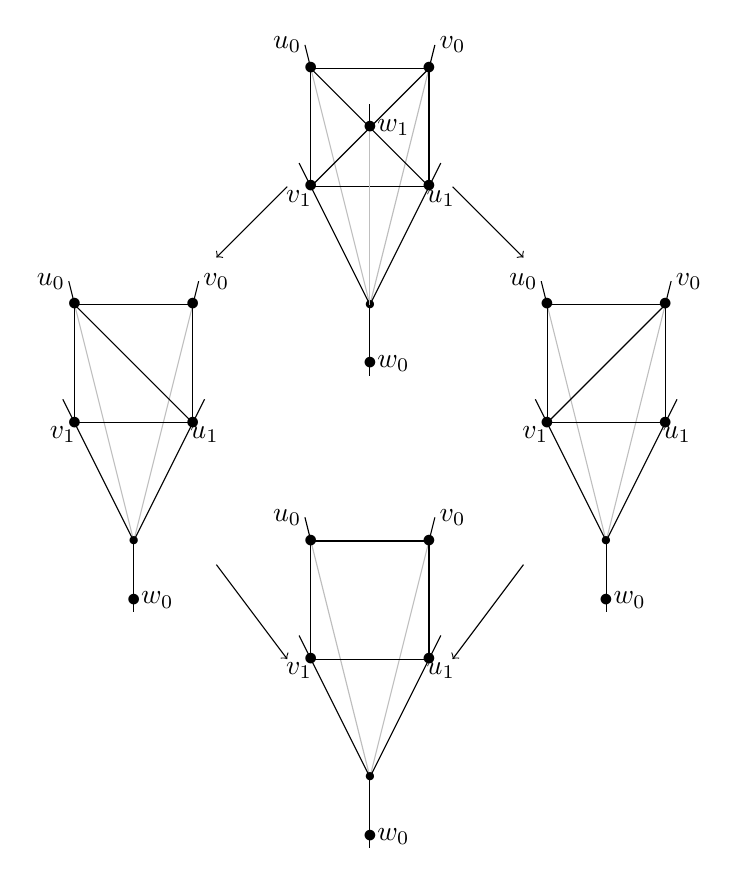
\begin{tikzpicture}[scale=1.5]
   \begin{scope} [xshift = 2cm, yshift=2cm]
   \draw[gray!50] (1/2,-1) -- (0,1) (1/2,-1) -- (1,1);
   \draw (1/2,-1) -- (0,0) (1/2,-1) -- (1,0);
   \draw (0,0) -- (1,0) -- (1,1) -- (0,1) -- cycle;
   \node at (0,0) {$\bullet$};
   \node at (-0.1,-0.1) {$v_{1}$};
   \node at (1,0) {$\bullet$};
   \node at (1.1,-0.1) {$u_{1}$};
   \node at (1,1) {$\bullet$};
   \node at (1.2,1.2) {$v_{0}$};
   \node at (0,1) {$\bullet$};
   \node at (-0.2,1.2) {$u_{0}$};
   \node at (1/2,-1) {\scriptsize $\bullet$};
   \draw (0,0) -- (-0.1,0.2);
   \draw (1,0) -- (1.1,0.2);
   \draw (0,1) -- (-0.05,1.2);
   \draw (1,1) -- (1.05,1.2);
   \draw (0.5,-1) -- (0.5,-1.6);
   \node at (0.5,-1.5) {$\bullet$};
   \node at (0.7,-1.5) {$w_{0}$};

   \draw[gray!50] (0.5,-1) -- (0.5,0.5);
   \draw (0.5,0.5) -- (0.5,0.7);
   \node at (0.5,0.5) {$\bullet$};
   \node at (0.7,0.5) {$w_{1}$};

   \draw (0,0) -- (1,1);
   \draw (0,1) -- (1,0);
   \end{scope}

 \draw[->] (1.8,2) to   (1.2,1.4);
 \draw[->] (3.2,2) to   (3.8,1.4);

   \begin{scope} [xshift = 4cm]
   \draw[gray!50] (1/2,-1) -- (0,1) (1/2,-1) -- (1,1);
   \draw (1/2,-1) -- (0,0) (1/2,-1) -- (1,0);
   \draw (0,0) -- (1,0) -- (1,1) -- (0,1) -- cycle;
   \node at (0,0) {$\bullet$};
   \node at (-0.1,-0.1) {$v_{1}$};
   \node at (1,0) {$\bullet$};
   \node at (1.1,-0.1) {$u_{1}$};
   \node at (1,1) {$\bullet$};
   \node at (1.2,1.2) {$v_{0}$};
   \node at (0,1) {$\bullet$};
   \node at (-0.2,1.2) {$u_{0}$};
   \node at (1/2,-1) {\scriptsize $\bullet$};
   \draw (0,0) -- (-0.1,0.2);
   \draw (1,0) -- (1.1,0.2);
   \draw (0,1) -- (-0.05,1.2);
   \draw (1,1) -- (1.05,1.2);
   \node at (0.5,-1.5) {$\bullet$};
   \node at (0.7,-1.5) {$w_{0}$};
   \draw (0.5,-1) -- (0.5,-1.6);
   
   \draw (0,0) -- (1,1);
   \end{scope}
   
   
   \begin{scope} [xshift = 0cm]
   \draw[gray!50] (1/2,-1) -- (0,1) (1/2,-1) -- (1,1);
   \draw (1/2,-1) -- (0,0) (1/2,-1) -- (1,0);
   \draw (0,0) -- (1,0) -- (1,1) -- (0,1) -- cycle;
   \node at (0,0) {$\bullet$};
   \node at (-0.1,-0.1) {$v_{1}$};
   \node at (1,0) {$\bullet$};
   \node at (1.1,-0.1) {$u_{1}$};
   \node at (1,1) {$\bullet$};
   \node at (1.2,1.2) {$v_{0}$};
   \node at (0,1) {$\bullet$};
   \node at (-0.2,1.2) {$u_{0}$};
   \node at (1/2,-1) {\scriptsize $\bullet$};
   \draw (0,0) -- (-0.1,0.2);
   \draw (1,0) -- (1.1,0.2);
   \draw (0,1) -- (-0.05,1.2);
   \draw (1,1) -- (1.05,1.2);
   \draw (0.5,-1) -- (0.5,-1.6);
   \node at (0.5,-1.5) {$\bullet$};
   \node at (0.7,-1.5) {$w_{0}$};
   
   \draw (0,1) -- (1,0);
   \end{scope}

  \draw[->] (1.2,-1.2) to (1.8,-2);
  \draw[->] (3.8,-1.2) to (3.2,-2);

   \begin{scope} [xshift = 2cm, yshift=-2cm]
   \draw[gray!50] (1/2,-1) -- (0,1) (1/2,-1) -- (1,1);
   \draw (1/2,-1) -- (0,0) (1/2,-1) -- (1,0);
   \draw (0,0) -- (1,0) -- (1,1) -- (0,1) -- cycle;
   \node at (0,0) {$\bullet$};
   \node at (-0.1,-0.1) {$v_{1}$};
   \node at (1,0) {$\bullet$};
   \node at (1.1,-0.1) {$u_{1}$};
   \node at (1,1) {$\bullet$};
   \node at (1.2,1.2) {$v_{0}$};
   \node at (0,1) {$\bullet$};
   \node at (-0.2,1.2) {$u_{0}$};
   \node at (1/2,-1) {\scriptsize $\bullet$};
   \draw (0,0) -- (-0.1,0.2);
   \draw (1,0) -- (1.1,0.2);
   \draw (0,1) -- (-0.05,1.2);
   \draw (1,1) -- (1.05,1.2);
   \draw (0.5,-1) -- (0.5,-1.6);
   \node at (0.5,-1.5) {$\bullet$};
   \node at (0.7,-1.5) {$w_{0}$};
   \end{scope}
\end{tikzpicture}
\label{fig!atiyah-flop}
\end{center}
\end{figure}

Note that by replacing $T$ with $\mathbb{P}^{r} \times \mathbb{P}^{s}$, it is easy to construct similarly examples in higher dimension.
\newpage
\section{toric varieties}
By Cox, we can construct following toric varieties.

Let $N=\mathbb{Z}^{r+s+1}$ be a lattice with basis of $u_{1},\ldots ,u_{s},e_{1},\ldots ,e_{r},e_{r+1} $

Then $X=X_\Sigma=\mathbb{P}(\mathcal{O}_{\mathbb{P}}^s\oplus {\mathcal{O}_{\mathbb{P}^s}(1)}^{\oplus (r+1)})$ is given by $\Sigma$ as following:
Let $u_{s+1}=-u_{1}+\cdots-u_{s}+e_{1}+\cdots+e_{r+1}\in N$ and $w=-e_{1}-\cdots-e_{r+1}=-u_{1}-\cdots -u_{s+1}$.
$\Sigma$ is induced by max  cones $\Sigma_{\max}$ consisting of 
\[
cone(w,u_{1},\ldots,\hat{u_i},\ldots,u_{s+1},e_{1},\ldots,\hat{e_{j}},\ldots,e_{r+1}), 0\leqslant i \leqslant s+1, 1 \leqslant j \leqslant r+1
\]
and 
\[
cone(u_{1},\ldots,\hat{u_{j}},\ldots,u_{s+1},e_{1},\ldots,e_{r+1}),1\leqslant i \leqslant s+1.
\]
Denote following toric invariant curves:
\begin{itemize}
  \item $L_{u,e}=cone(u_{1},\ldots ,u_{s},e_{1},\ldots ,e_{r})$;
  \item $L_{e,w}=cone(w,u_{1},\ldots ,u_{s},e_{1},\ldots ,e_{r+1})$;
  \item $L_{u,w}=cone(w,u_{1},\ldots ,u_{s+1},e_{1},\ldots ,e_{r})$;
  \item $L_{e}=cone(u_{1},\ldots ,u_{s},e_{1},\ldots ,e_{r+1})$;
\end{itemize}
Let $D_{i}$ be the toric divisors corresponding to $u_{i}$ and $E_{j}$ corresponding to $e_{j}$. Let $W$ be the toric divisors corresponding to $w$.  Then the intersecting numbers are as following. 

\begin{tabular}{lllll}
           & $D_{i}$ & $E_{j}$  & $W$   \\
 $L_{u,e}$ & $0$     & $1$      & $1$   \\
 $L_{e,w}$ & $1$     & $0$      & $1$   \\
 $L_{u,w}$ & $0$     & $1$      & $1$   \\
 $L_{e}$   & $1$     & $-1$     & $0$   
\end{tabular}

  
Note that $L_{u,e}\equiv L_{u,w}$ and $D_{i}+E_{j}\sim W$.

Similarly, we can construct $X'=X_{\Sigma'}=\mathbb{P}(\mathcal{O}_{\mathbb{P}}^r\oplus {\mathcal{O}_{\mathbb{P}^r}(1)}^{\oplus (s+1)})$ as following.
Let $e_{s+1}'=-e_{1}'-\cdots-e_{s}+u_{1}'+\cdots+u_{r+1}'\in N'$ and $w'=-u_{1}'-\cdots-u_{s+1}'=-e_{1}'-\cdots -e_{r+1}'$.
Let $\Sigma'$ be a fan in $N'$ induced by max cones $\Sigma_{\max}'$ consisting of 
\[
cone(w',e_{1}',\ldots,\hat{e_i'},\ldots,e_{r+1}',u_{1}',\ldots,\hat{u_{j}'},\ldots,u_{s+1}'), 0\leqslant i \leqslant r+1, 1 \leqslant j \leqslant s+1
\]
and 
\[
cone(e_{1}',\ldots, \hat{e_{j}'} , \ldots ,e_{r+1}',u_{1}',\ldots,u_{s+1}'),1\leqslant j \leqslant r+1.
\]
There is an isomorphism $\phi:N'\to N$ given by
\[
w'\to w,u_i'\to u_i, e_j'\to e_j, 1\leqslant i \leqslant s+1,1\leqslant j \leqslant s+1.
\]
Let $\Sigma^+$ be the image of $\Sigma'$ under $\phi$ in $N$, and $X^+=X(\Sigma^+)\cong X'$. Then $\Sigma^+$ is induced by max cones $\Sigma^+_{\max}$ consisting of 
\[
cone(w,u_{1},\ldots,\hat{u_i},\ldots,u_{s+1},e_{1},\ldots,\hat{e_{j}},\ldots,e_{r+1}), 0\leqslant i \leqslant s+1, 1 \leqslant j \leqslant r+1
\]
and 
\[
cone(u_{1},\ldots,u_{s+1},e_{1},\ldots,\hat{e_j},\ldots,e_{r+1}),1\leqslant i \leqslant s+1.
\]
The section $\mathbb{P}^s\hookrightarrow X$ is induced by the cone
\[
cone(e_1,\ldots,e_{r+1}),
\]
and  the section $\mathbb{P}^r\hookrightarrow X^+$ is induced by the cone
\[
cone(u_1,\ldots,u_{s+1}).
\]
Moreover, Let $V=X(\Sigma_V)$ be a singular variety, where $\Sigma_V$ is induced by $\Sigma_{V,\max}$ consisting of 
\[
cone(w,u_{1},\ldots,\hat{u_i},\ldots,u_{s+1},e_{1},\ldots,\hat{e_{j}},\ldots,e_{r+1}), 0\leqslant i \leqslant s+1, 1 \leqslant j \leqslant r+1
\]
and 
\[
cone(u_{1},\ldots,u_{s+1},e_{1},\ldots,\ldots,e_{r+1}).
\]
Note that the singular point $P$ corresponds to the cone
\[
cone(u_{1},\ldots,u_{s+1},e_{1},\ldots,\ldots,e_{r+1}).
\]
Furthermore, $X\to V$ is the small contraction which maps the section $\mathbb{P}^s$ to $P$ and $X^+\to V$ is the small contraction which maps the section $\mathbb{P}^r$ to $P$. In fact, we have
\[ K_X.L_s=r-s,K_{X^+}.L_r=s-r\]
where $L_s$ is the line in the section $\mathbb{P}^s$ and $L_r$ is the line in the section $\mathbb{P}^r$. Therefore, $X \dashrightarrow X^+$ is a $K_X$-flip if $r<s$ and is a $K_X$-flop if $r=s$.
When $r=s=1$, this is the classic Atiyah flop.

On the other hand, let $Y\to V$ be the blowing up of point $P \in V$, then $Y$ is a toric variety given by $\Sigma_{Y}$ in $N$, where $\Sigma_{Y,\max}$ consisting of
\[
  cone(w,u_{1},\ldots ,\hat{u_{i}},\ldots ,u_{s+1},e_{1},\ldots ,\hat{e_{j}},\ldots ,e_{r+1})
\]
and
\[
  cone(-w,u_{1},\ldots ,\hat{u_{i}},\ldots ,u_{s+1},e_{1},\ldots ,\hat{e_{j}},\ldots ,e_{r+1})
\]
The exceptional divisor $E\cong \mathbb{P}^{r} \times \mathbb{P}^{s}$ corresponds to $1$-dimensional cone generated by $-w$. Moreover, there are two divisorial contractions $Y\to X$ and $Y\to X^{+}$, corresponding to two projections of $E$.
Moreover, Let $T=\mathbb{P}^{r} \times \mathbb{P}^{s}$, then $Y\cong \mathbb{P}(\mathcal{O}_{T}\oplus\mathcal{O}_{T}(1))$.
Denote following toric invariant curves:
\begin{itemize}
  \item $L_{u,e}=cone(u_{1},\ldots ,u_{s},e_{1},\ldots ,e_{r})$;
  \item $L_{e,w}=cone(w,u_{1},\ldots ,u_{s},e_{1},\ldots ,e_{r+1})$;
  \item $L_{u,w}=cone(w,u_{1},\ldots ,u_{s+1},e_{1},\ldots ,e_{r})$;
  \item $L_{e,-w}=cone(-w,u_{1},\ldots ,u_{s},e_{1},\ldots ,e_{r+1})$;
  \item $L_{u,-w}=cone(-w,u_{1},\ldots ,u_{s+1},e_{1},\ldots ,e_{r})$;
\end{itemize}
Let $D_{i}$ be the toric divisors corresponding to $u_{i}$ and $E_{j}$ corresponding to $e_{j}$. Let $W$ be the toric divisors corresponding to $w$ and $F$ corresponding to $-w$.  Then the intersecting numbers are as following. 

\begin{table}[]
\begin{tabular}{lllll}
           & $D_{i}$ & $E_{j}$  & $W$ & $F$       \\
 $L_{u,e}$ & $0$     & $0$      & $1$ & $1$  \\
 $L_{e,w}$ & $1$     & $0$      & $1$ & $0$  \\
 $L_{u,w}$ & $0$     & $1$      & $1$ & $0$  \\
 $L_{e,-w}$ & $1$     & $0$      & $0$ & $-1$  \\
 $L_{u,-w}$ & $0$     & $1$      & $0$ & $-1$  \\
\end{tabular}
\end{table}

Note that $L_{u,e}+L_{u,-w}\equiv L_{u,w},L_{u,e}+L_{e,-w}\equiv L_{e,w}$ and $D_{i}+E_{j}+F\sim W$.

\section{toric foliations}
Let $X=X_{\Sigma}$ be a toric variety defined by a fan $\Sigma$ in a lattice $N$. Suppose $N' \subset N$ is a sublatice, and let $W=N' \times \mathbb{C},\bar{N}=N/N'$. Then there is a morphism $f:T_{N} \to T_{\bar{N}}$ between toruses. Let $\mathcal{F}$ be the foliation induced by $f$, then $\mathcal{F}$ is algebraically integrable, and 
\[
  K_{\mathcal{F}}=-\sum_{\rho \subset W}D_{\rho}.
\]
Moreover, a Divisor $D_{\rho}$ is $\mathcal{F}$-invariant   if and only if $\rho \not\subset W$.

\section{foliation flop example}
Let $X$ and $X^{+}$ be the varieties defined as before. Let $N_{\mathcal{F}}$ be the sublattice of $N$ generated by
\[
  e_{1},\ldots ,e_{m},u_{1},\ldots ,u_{m},0\leqslant m \leqslant \min \{s,r\}.
\]
Then $K_{\mathcal{F}}=-\sum_{i=1}^{m}D_{e_{i}}-\sum_{i=1}^{m}D_{u_{i}}$, therefore
\[
  K_{\mathcal{F}}.L_{s}=K_{\mathcal{F}}.L_{r}=0.
\]
Thus $X\dashrightarrow X^{+}$ is a $K_{\mathcal{F}}$-flop.


\end{document}
